\documentclass[12pt]{beamer}
\usetheme{Pittsburgh}
\usecolortheme{seagull}
\usepackage[utf8]{inputenc}
\usepackage[english]{babel}
\usepackage{amsmath}
\usepackage{amsfonts}
\usepackage{amssymb}
\usepackage{graphicx}
\author{Design and Verification of Security Protocols and Security Ceremonies}
\title{Lecture Plan Overview}
%\setbeamercovered{transparent} 
\setbeamertemplate{navigation symbols}{} 
%\logo{
\includegraphics[scale=0.015]{Brasao_UFSC.png}
\includegraphics[scale=0.2]{brasao_PPGCC.jpg}} 
\institute{Programa de Pós-Graduacão em Ciências da Computacão \\ Dr. Jean Everson Martina} 
\date{\vspace{.2cm}August-November 2016} 
\subject{} 
\usebackgroundtemplate{
\includegraphics[width=\paperwidth,
height=\paperheight]{../reusable_images/fundo_UFSC.png}}
\begin{document}

{
\usebackgroundtemplate{
\includegraphics[width=\paperwidth,
height=\paperheight]{../reusable_images/fundo_capa.png}}
\begin{frame}
\titlepage

\includegraphics[scale=0.3]{../reusable_images/brasao_PPGCC.jpg}
\end{frame}
}


%\begin{frame}
%\tableofcontents
%\end{frame}

\begin{frame}{Course Identification}
\begin{itemize}
\item INE 410128 - Design and Verification of Security Protocols and Security
Ceremonies \pause
\item 3 credits – 45 hours \pause
\item Dr. Jean Everson Martina 
\end{itemize}
\end{frame}

\begin{frame}{About the Lecturer}
\begin{columns}
\column{.5\textwidth}
\begin{center}
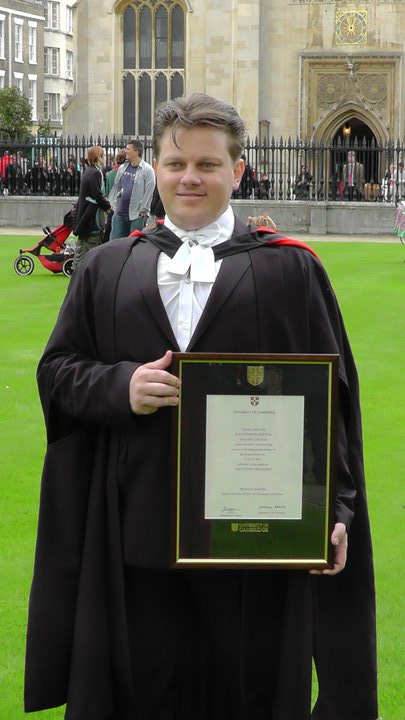
\includegraphics[scale=0.26]{academic_dress.jpg}
\end{center}
\column{.5\textwidth}
\begin{itemize}
\item B.Sc. In CompSci;\pause
\item M.Sc. In CompSci;\pause
\item Ph.D. In CompSci;\pause
\item Several International Projects; \pause
\item Working on Cryptography, Digital Signatures, Security Protocols and Security Ceremonies.
\end{itemize}
\end{columns}
\end{frame}

\begin{frame}{About the Students}
I would like to know:
\begin{itemize}
\item Your Name and Affiliation;\pause
\item Academic Background;\pause
\item Interests in Security;\pause
\item Prior knowledge on Security;\pause
\item Anything else you believe is important to share.
\end{itemize}
\end{frame}


\begin{frame}{Course Prerequisites}
\begin{itemize}
\item There are no prerequisites for this course;\pause
\item Some prior familiarity with cryptography is good;\pause
\item Some prior familiarity with formal methods may be helpful;\pause
\item All necessary background will be covered in class.
\end{itemize}
\end{frame}

\begin{frame}{Study Aims}
\begin{itemize}
\item Cryptographic Primitives;\pause
\item Security Properties;\pause
\item Classical Protocols;\pause
\item Threat Modelling;\pause
\item Protocol Verification Techniques;\pause
\item Advanced Security Protocols;\pause
\item Advanced Security Ceremonies;\pause
\item Formal Verification of Security Protocols and Security Ceremonies.
\end{itemize}
\end{frame}

\begin{frame}{General Objective}

{\Large Understand the concepts of security protocols and security ceremonies design and verification.}

\end{frame}

\begin{frame}{Specific Objectives}
\begin{itemize}
\item Understand security primitives as a way of yielding security;\pause
\item Understand the relation between the different security properties and their
compositions;\pause
\item Review classical security protocols;\pause
\item Understand the different threat models available for symbolic evaluation of security protocols and security ceremonies;
\end{itemize}
\end{frame}

\begin{frame}{Specific Objectives}
\begin{itemize}
\item Understand the security verification techniques available today;\pause
\item Study advanced security protocols;\pause
\item Study advanced security ceremonies;\pause
\item Be able to apply formal verification techniques based on theorem provers on security protocols and security ceremonies.
\end{itemize}
\end{frame}


\begin{frame}{Course Outline}
\begin{itemize}
\item Cryptographic Primitives;\pause
\item Security Properties;\pause
\item Classical Protocols;\pause
\item Threat Modelling;\pause
\item Protocol Verification Techniques;\pause
\item Advanced Security Protocols;\pause
\item Advanced Security Ceremonies;\pause
\item Formal Verification of Security Protocols and Security Ceremonies.
\end{itemize}
\end{frame}


\begin{frame}{Methodology}
\begin{itemize}
\item The first part of the course will survey contemporary security protocols and their properties, including confidentiality, authentication, secure group communication, privacy, and anonymity. \pause
\item We will also cover cryptographic primitives, as well as standard formal models and tools used for mechanized verification of secure systems.
\end{itemize}
\end{frame}


\begin{frame}{Methodology}
The second part of the course will focus primarily on student projects, carried out individually or in small teams. A typical project may involve:\pause
\begin{itemize}
\item Coming up with a security specification for a particular system and performing a detailed analysis of its properties; or\pause
\item Extending an existing tool or method to support analysis of a new class of security properties; or\pause
\item Conducting a theoretical study of the relationship between several models.
\end{itemize}
\end{frame}

\begin{frame}{Studying Strategies}
\begin{itemize}
\item We will a series of classical papers on the area;\pause
\item Students are expected to have read the assignments for the week;\pause
\item The off-class workload for this course is about 90 hours;\pause
\item Some lectures will be open discussions regarding the topics.
\end{itemize}
\end{frame}

\begin{frame}{Important to Notice!}
\begin{itemize}
\item Lectures will be given in English;\pause
\item The course may be joined by international partners;\pause
\item Experts on the field will be invited to speak in some guest lectures;\pause
\item All the students will be required to join the virtual lecture room at the required time;\pause
\item The student MUST HAVE A WEBCAM for all the meetings so that participation can be attested;\pause
\item All the meetings will be recorded;\pause
\item This Course follows all UFSC regulations regarding regular courses.
\end{itemize}
\end{frame}

\begin{frame}{Evaluation}
\begin{itemize}
\item A final technical report written by the student;\pause
\item The technical report will be assessed using standard strategies used to evaluate conference papers;\pause
\item The technical reports will be evaluated over their readability, adherence to the
proposed topic, contribution, coherence of the experimentation conducted and the results achieved;\pause
\item Technical reports with a pass mark should be fit for submission to the main conferences in the area of security protocols, formal methods or foundations of computer security.
\end{itemize}
\end{frame}

\begin{frame}{Schedule}
\begin{itemize}
\item Tuesday 11:00-12:30 (BRT)
\item Thursday 11:00-12:30 (BRT)\pause
\item International participants should be aware that:
\begin{itemize}
\item Time shifts during the semester
\item Your summer time will end (usually -1 hour);
\item Brazil's summer time starts on the first Sunday of October (it will shift us 1 hour forward);
\end{itemize}
\end{itemize}
\end{frame}

\begin{frame}{Bibliography}
\begin{itemize}
\item Formal Correctness of Security Protocols. Bella, G.. 2007. Springer
\item Threat Modelling: Designing for Security. Shostack, A.. 2014. Wiley
\item Isabelle/HOL: A Proof Assistant for Higher-Order Logic. Nipkow, T. and Paulson, L.C. and Wenzel, M.. 2003. Springer Berlin Heidelberg
\end{itemize}
\end{frame}

{
\usebackgroundtemplate{
\includegraphics[width=\paperwidth,
height=\paperheight]{../reusable_images/fundo_capa.png}}
\begin{frame}

{\LARGE Questions????}

\end{frame}
}

\end{document}